% !TeX root = RJwrapper.tex
\title{Partitioned Local Depth (PaLD) Community Analyses in R}
\author{by Lucy D'Agostino McGowan, Katherine Moore, and Kenneth Berenhaut}

\maketitle

\abstract{%
Partitioned Local Depth (PaLD) is a framework for holistic consideration
of community structure for distance-based data. This paper describes an
R package, \CRANpkg{pald}, for calculating Partitioned Local Depth
(PaLD) probabilities, implementing community analyses, and creating data
visualizations to display community structure. We describe how to use
the package, walk through several examples, and discuss the approach in
relation to commonly used techniques.
}

\hypertarget{introduction}{%
\subsection{Introduction}\label{introduction}}

Partitioned Local Depth (PaLD) is a framework for holistic consideration
of community structure for distance-based data. Leveraging a socially
inspired perspective, the method provides network-based community
information which is founded on a new measure of local depth and
pairwise cohesion (partitioned local depth). The method does not require
distributional assumptions, optimization criteria, nor extraneous
inputs. A complete description of the perspective, together with a
discussion of the underlying social motivation, theoretical results, and
applications to additional data sets is provided in
\citet{berenhaut2022social}.

Building on existing approaches to (global) depth, local depth expresses
features of centrality via an interpretable probability which is free of
parameters and robust to outliers. Then, partitioning the probability
which defines local depth, we obtain a measure of cohesion between pairs
of individuals. Both local depth and cohesion reflect aspects of
relative position (rather than absolute distance) and provide a
straightforward way to account for varying density across the space. As
shown in \citet{berenhaut2022social}, provided that two sets are
separated (in the sense that the minimum between-set distance is greater
than the maximum within-set distance), cohesion is invariant under the
contraction and dilation of the distances within each set. This property
may be particularly valuable when one has reason to believe that there
is heterogeneity in density across the space.

As cohesion captures a sense of the relationship strength between
points, we can then visualize the resulting community structure with a
network whose edges are weighted by (mutual) cohesion. The underlying
social framework motivates a straightforward yet elegant threshold for
distinguishing between strongly and weakly cohesive pairs.

Networks obtained from cohesion can be displayed using a force-directed
graph drawing algorithm; here, we will graphically emphasize strong ties
(colored by connected component). We refer to the connected components
of the network of strong ties as community ``clusters.'' Note that to
qualify as a cluster in this definition, one may not have any strong
ties with those outside the cluster, and thus the existence of disjoint
groups is a strong signal for separation. Here, clusters are identified
without additional user inputs nor optimization criteria. If one wishes
to further break the community graph into groups, one may consider using
community detection methods (such as spectral clustering or the Louvain
algorithm), as available, say, in the \CRANpkg{igraph} package. One may
also use the collection of strong ties in place of (weighted)
\(k\)-nearest neighbors in settings such as classification and
smoothing. Overall, the structural information obtained from local
depth, cohesion and community graphs can provide a holistic perspective
to the data which does not require the use of distributional
assumptions, optimization criteria nor additional user inputs.

We present a new package, \CRANpkg{pald}, for calculating Partitioned
Local Depth (PaLD) probabilities, implementing community analyses, and
creating data visualizations to display community structure. This paper
describes how to use the package, walks through several examples, and
discusses the approach in the context of commonly used techniques,
demonstrating both the novelty of the method and utility of the
implementation in the package described.

\hypertarget{pald}{%
\subsection{pald}\label{pald}}

The main functions in the \CRANpkg{pald} package can be split into 3
categories:

\begin{enumerate}
\def\labelenumi{\arabic{enumi}.}
\tightlist
\item
  A function for computing the cohesion matrix
\item
  Functions for extracting useful information from the cohesion matrix,
  such as local depths, neighbors, community clusters, and graph objects
\item
  Plotting functions for community graphs
\end{enumerate}

In addition, the package provides a number of pertinent example data
sets which may be used to demonstrate community analysis, including a
synthetic data set of two-dimensional points created by
\citet{gionis1clustering} to demonstrate aggregation, clustering data
generated from the scikit-learn Python package
\citep{pedregosa2011scikit}, data describing cognate relationships
between words across 87 Indo-European languages \citep{dyen92}, data
compiled by \cite{tissue} of tissue gene expressions, data emplying
information from the World Values Survey \citep{inglehart2014world} on
cultural values regarding family, religion, education, and institutions
for several regions \citep{muthukrishna2020beyond}, and three example
data sets generated for the \citet{berenhaut2022social} paper.

While it is not a necessity, the \CRANpkg{pald} package is designed to
function well with the pipe operator, \texttt{\textbar{}\textgreater{}}.
This functionality will be demonstrated below.

\hypertarget{creating-the-cohesion-matrix}{%
\subsubsection{Creating the cohesion
matrix}\label{creating-the-cohesion-matrix}}

For the purposes of the \CRANpkg{pald} package, the sole input for the
Partitioned Local Depth (PaLD) computations is a distance matrix or
\texttt{dist} object. Note that the collection of input distances (or
dissimilarities) does not need to satisfy the triangle inequality nor be
symmetric. More generally, the method only requires triplet distance
comparisons, as opposed to exact numeric distances (see
\citet{berenhaut2022social}).

For demonstration purposes, we first show how one can compute a distance
matrix from an input data frame with, say, two variables \texttt{x1} and
\texttt{x2}. The input data may be of any dimension; in fact the PaLD
framework provides advantages when considering high-dimensional data
(see the \textbf{Examples} section as well as
\citet{berenhaut2022social}).

\begin{Schunk}
\begin{Sinput}
library(pald)
df <- data.frame(
  x1 = c(6, 8, 8, 16, 4, 14),
  x2 = c(5, 4, 10, 8, 4, 10)
)
rownames(df) <- c("A", "B", "C", "D", "E", "F")
\end{Sinput}
\end{Schunk}

The \texttt{dist} function returns a (default Euclidean) pairwise
distance matrix for an input data frame, as demonstrated below. If the
data are already provided as a distance matrix (or \texttt{dist}
object), the user can skip to the next step. Note that the distance
matrix needed for the subsequent functions does not need to be a
\texttt{dist} object and \emph{need not} be symmetric.

\begin{Schunk}
\begin{Sinput}
d <- dist(df)
\end{Sinput}
\end{Schunk}

The function above creates a \texttt{dist} object. If converted to a
matrix, this will be an \(n\times n\) distance matrix, where \(n\)
corresponds to the number of observations in the original data frame (in
this example \(n = 6\)).

This \texttt{dist} object, or a distance matrix, can then be passed to
the \texttt{cohesion\_matrix} function in order to calculate pairwise
cohesion values.

Cohesion is an interpretable probability that reflects the strength of
alignment of two points within local regions. It captures aspects of the
relative positioning of points and accounts for varying density across
the space (see \citet{berenhaut2022social}).

\begin{Schunk}
\begin{Sinput}
d <- dist(df)
cohesion_matrix(d)
\end{Sinput}
\begin{Soutput}
#>            A          B          C         D          E         F
#> A 0.25000000 0.18333333 0.06666667 0.0000000 0.18333333 0.0000000
#> B 0.14000000 0.24000000 0.05000000 0.0000000 0.10666667 0.0000000
#> C 0.07333333 0.07333333 0.20333333 0.0000000 0.03333333 0.0800000
#> D 0.00000000 0.00000000 0.00000000 0.2333333 0.00000000 0.1333333
#> E 0.14000000 0.10666667 0.03333333 0.0000000 0.24000000 0.0000000
#> F 0.00000000 0.00000000 0.05000000 0.1400000 0.00000000 0.2400000
#> attr(,"class")
#> [1] "cohesion_matrix" "matrix"          "array"
\end{Soutput}
\end{Schunk}

Equivalently, the user can use the native pipe
\texttt{\textbar{}\textgreater{}} as follows.

\begin{Schunk}
\begin{Sinput}
df |>
  dist() |>
  cohesion_matrix()
\end{Sinput}
\begin{Soutput}
#>            A          B          C         D          E         F
#> A 0.25000000 0.18333333 0.06666667 0.0000000 0.18333333 0.0000000
#> B 0.14000000 0.24000000 0.05000000 0.0000000 0.10666667 0.0000000
#> C 0.07333333 0.07333333 0.20333333 0.0000000 0.03333333 0.0800000
#> D 0.00000000 0.00000000 0.00000000 0.2333333 0.00000000 0.1333333
#> E 0.14000000 0.10666667 0.03333333 0.0000000 0.24000000 0.0000000
#> F 0.00000000 0.00000000 0.05000000 0.1400000 0.00000000 0.2400000
#> attr(,"class")
#> [1] "cohesion_matrix" "matrix"          "array"
\end{Soutput}
\end{Schunk}

The \emph{cohesion matrix} output by the \texttt{cohesion\_matrix}
function is the main input for the majority of the remaining functions.

\hypertarget{functions-for-extracting-information-from-the-cohesion-matrix}{%
\subsubsection{Functions for extracting information from the cohesion
matrix}\label{functions-for-extracting-information-from-the-cohesion-matrix}}

From the \emph{cohesion matrix}, a variety of useful quantities can be
computed. Below, we create a cohesion matrix using the functions
described in the previous section.

\begin{Schunk}
\begin{Sinput}
df |>
  dist() |>
  cohesion_matrix() -> cohesion
\end{Sinput}
\end{Schunk}

The \texttt{local\_depths} function calculates the \emph{depth} of each
point, outputting a vector of local depths. Local depth is an
interpretable probability which reflects aspects of relative position
and centrality via distance comparisons (e.g., \(d(z, x) < d(z, y)\),
see \citet{berenhaut2022social}).

\begin{Schunk}
\begin{Sinput}
local_depths(cohesion)
\end{Sinput}
\begin{Soutput}
#>         A         B         C         D         E         F
#> 0.6833333 0.5366667 0.4633333 0.3666667 0.5200000 0.4300000
\end{Soutput}
\end{Schunk}

In this case, the deepest point is \texttt{A}.

The \texttt{strong\_threshold} function will calculate the cohesion
threshold for strong ties, which reflects typical cohesion for local
points (see \citet{berenhaut2022social}). Computationally, this is equal
to half the average of the diagonal of the cohesion matrix, and is a
threshold that may be used to distinguish between strong and weak ties.

\begin{Schunk}
\begin{Sinput}
strong_threshold(cohesion)
\end{Sinput}
\begin{Soutput}
#> [1] 0.1172222
\end{Soutput}
\end{Schunk}

In this case, the threshold is a little above \texttt{0.117}.

The function \texttt{cohesion\_strong} will update the cohesion matrix
to set all weak ties to zero (via the \texttt{strong\_threshold}
function). Optionally, the matrix will also be symmetrized, using the
entry-wise (parallel) minimum of the cohesion matrix and its transpose,
with the default parameter \texttt{symmetric\ =\ TRUE}.

\begin{Schunk}
\begin{Sinput}
cohesion_strong(cohesion)
\end{Sinput}
\begin{Soutput}
#>      A    B         C         D    E         F
#> A 0.25 0.14 0.0000000 0.0000000 0.14 0.0000000
#> B 0.14 0.24 0.0000000 0.0000000 0.00 0.0000000
#> C 0.00 0.00 0.2033333 0.0000000 0.00 0.0000000
#> D 0.00 0.00 0.0000000 0.2333333 0.00 0.1333333
#> E 0.14 0.00 0.0000000 0.0000000 0.24 0.0000000
#> F 0.00 0.00 0.0000000 0.1333333 0.00 0.2400000
#> attr(,"class")
#> [1] "cohesion_matrix" "matrix"          "array"
\end{Soutput}
\end{Schunk}

The \texttt{community\_graphs} function takes the cohesion matrix and
creates \CRANpkg{igraph} objects, graphs that describe the (symmetrized)
relationship structure between points. This function will output a list
of three objects:

\begin{itemize}
\tightlist
\item
  \texttt{G}: the weighted (community) graph whose edge weights are
  mutual cohesion
\item
  \texttt{G\_strong}: the weighted (community) graph consisting of edges
  for which mutual (symmetrized) cohesion (i.e.~the minimum of the two
  directed cohesion values for any given pair) is greater than the
  threshold for strong ties
\item
  \texttt{layout}: the graph layout. By default this is provided by the
  Fruchterman Reingold (FR) force-directed graph drawing algorithm for
  the graph \texttt{G}, as implemented in the \CRANpkg{igraph} package.
\end{itemize}

\begin{Schunk}
\begin{Sinput}
graphs <- community_graphs(cohesion)
graphs[["G_strong"]]
\end{Sinput}
\begin{Soutput}
#> IGRAPH 5de0378 UNW- 6 3 --
#> + attr: name (v/c), weight (e/n)
#> + edges from 5de0378 (vertex names):
#> [1] A--B A--E D--F
\end{Soutput}
\end{Schunk}

Here we see that there are three connected components, ties \texttt{A-B}
and \texttt{A-E} form the first community cluster, and the tie
\texttt{D-F} which forms another.

The \texttt{any\_isolated()} function will check whether there are any
isolated points (according to cohesion).

\begin{Schunk}
\begin{Sinput}
any_isolated(cohesion)
\end{Sinput}
\end{Schunk}

\noindent Here, there are no isolated points, i.e.~points having zero
cohesion with all other points in the data (an extreme form of outlier).

The ``community clusters'' identified by PaLD are the connected
components of the graph of strong ties, \texttt{G\_strong}. To directly
calculate these, we can use the \texttt{community\_clusters} function.
This will output a data frame with two columns; the first corresponds to
the \texttt{point}, as identified by the row name of the original input
data frame, \texttt{df}, the second identifies the \texttt{community}
that the point belongs to.

\begin{Schunk}
\begin{Sinput}
community_clusters(cohesion)
\end{Sinput}
\begin{Soutput}
#>   point community
#> A     A         1
#> B     B         1
#> C     C         2
#> D     D         3
#> E     E         1
#> F     F         3
\end{Soutput}
\end{Schunk}

In this example, three communities are identified with these six points.
Points \texttt{A}, \texttt{B}, and \texttt{E} fall into Community 1.
Point \texttt{C} is in Community 2 (a community of size 1) and points
\texttt{D} and \texttt{F} fall into Community 3.

\hypertarget{plotting-functions}{%
\subsection{Plotting functions}\label{plotting-functions}}

The final category of function is that for data visualization. We can
begin by visualizing the points in the data frame \texttt{df} (Figure
\ref{fig:fig1}). When visualizing these points, it is important to have
the aspect ratio of the x and y axes equal to 1 so as to not distort
distances. When using the \CRANpkg{ggplot2} package for this
visualization, one can use the command
\texttt{coord\_fixed(ratio\ =\ 1)}. If using the \texttt{plot} function
included in the base library, one can use the \texttt{asp\ =\ 1}
argument.

\begin{Schunk}
\begin{Sinput}
library(ggplot2)
ggplot(df, aes(x1, x2)) +
  geom_text(label = rownames(df)) +
  coord_fixed(ratio = 1) +
  xlim(c(4, 16)) +
  ylim(c(4, 16))
\end{Sinput}
\begin{figure}[H]
\begin{center}
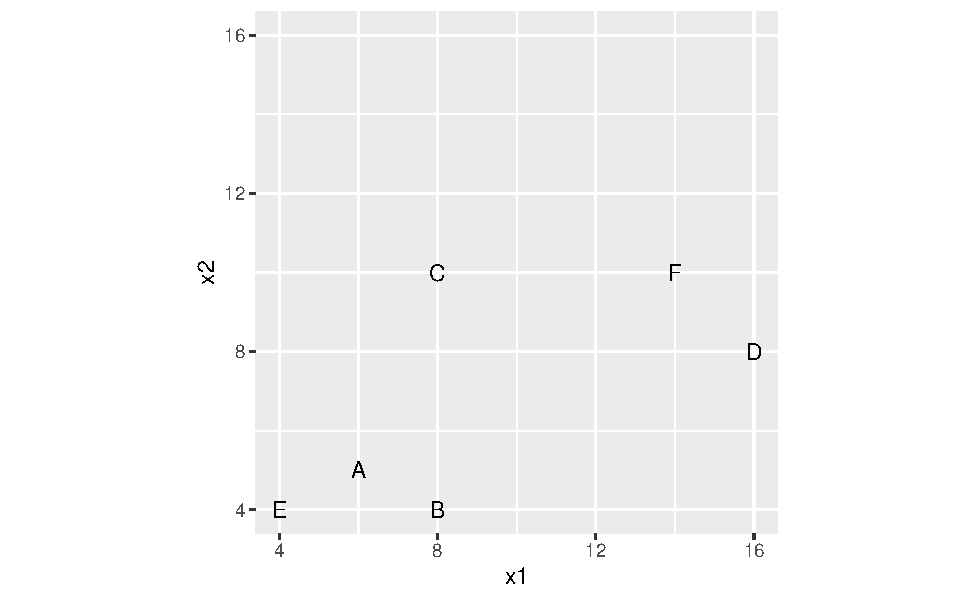
\includegraphics[width=5in]{dagostino-mcgowan_files/figure-latex/fig1-1} \caption[Visualization of the points from the data frame `df`]{Visualization of the points from the data frame `df`}\label{fig:fig1}
\end{center}
\end{figure}
\end{Schunk}

We can pass the cohesion matrix to the \texttt{plot\_community\_graphs}
function to view the relationship between points (Figure
\ref{fig:fig2}). The function will also permit parameters that can be
passed to \texttt{plot.igraph} via the \texttt{...} argument.

\begin{Schunk}
\begin{Sinput}
plot_community_graphs(cohesion,
                      vertex.label.cex = 2,
                      vertex.label.dist = 0.9)
\end{Sinput}
\begin{figure}[H]
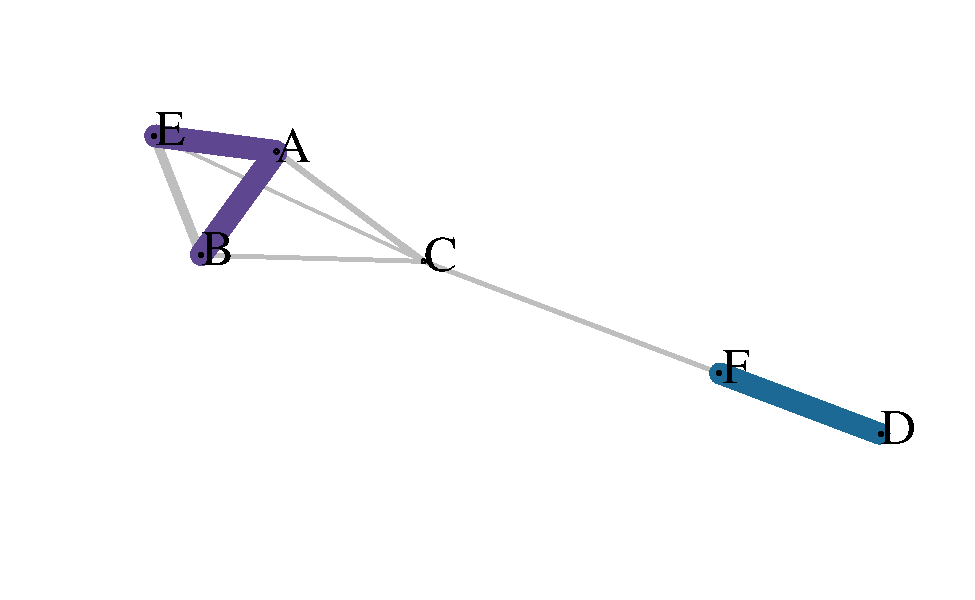
\includegraphics[width=5in,trim=0in 1in 0in 0.7in,clip]{dagostino-mcgowan_files/figure-latex/fig2-1} \caption[PaLD graph displaying the relationship between the points in data frame `df`]{PaLD graph displaying the relationship between the points in data frame `df`}\label{fig:fig2}
\end{figure}
\end{Schunk}

Notice in this plot the force-directed layout does not match that of the
original data frame as seen in Figure \ref{fig:fig1}. Since our original
data is two-dimensional, it may be reasonable to use the latter as the
layout for plotting. Figure \ref{fig:fig3} includes this update as well
as others addressing some of the aesthetics, such as employing more
readable labels. The \texttt{layout} argument allows the user to pass a
matrix to dictate the 2-dimensional layout of the graph. For example, if
we wanted the graph to match the visualization displayed in Figure
\ref{fig:fig1}, we could pass \texttt{as.matrix(df)} (a matrix of the
data frame \texttt{df}) to the \texttt{layout} argument (Figure
\ref{fig:fig3}). Here, we increase the vertex size and change the vertex
label color, through the argument specifications
\texttt{vertex.size\ =\ 100} and
\texttt{vertex.label.color\ =\ "white"}. Additionally, to allow axes, we
use \texttt{axes\ =\ TRUE}, and to put these back on the original scale
we set \texttt{rescale\ =\ FALSE}, resetting the axis limits using
\texttt{xlim} and \texttt{ylim}. The \texttt{par(pty\ =\ "s")} function
forces the subsequent plot to be square.

\begin{Schunk}
\begin{Sinput}
par(pty = "s")

plot_community_graphs(cohesion,
                      layout = as.matrix(df),
                      vertex.size = 100,
                      vertex.label.color = "white",
                      axes = TRUE,
                      rescale = FALSE,
                      asp = 1,
                      xlim = c(4, 16),
                      ylim = c(4, 16))
\end{Sinput}
\begin{figure}[H]
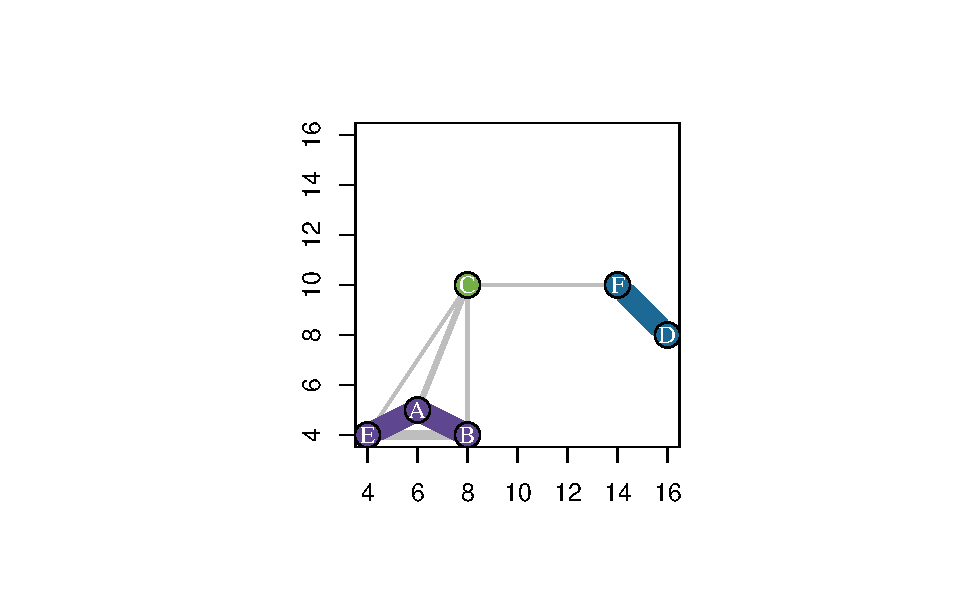
\includegraphics[width=5in,trim=0in 0.6in 0in 0.8in,clip]{dagostino-mcgowan_files/figure-latex/fig3-1} \caption[PaLD graph displaying the relationship between the points in data frame `df`, matching the original layout in Figure 1]{PaLD graph displaying the relationship between the points in data frame `df`, matching the original layout in Figure 1}\label{fig:fig3}
\end{figure}
\end{Schunk}

\hypertarget{examples}{%
\subsection{Examples}\label{examples}}

We will demonstrate the utility of the \CRANpkg{pald} package through
several illustrative examples.

\hypertarget{community-analysis-for-tissue-gene-expression-data}{%
\subsubsection{Community analysis for tissue gene expression
data}\label{community-analysis-for-tissue-gene-expression-data}}

The first example is from a subset of data from \citet{zilliox2007gene},
\citet{mccall2011gene}, and \citet{mccall2014gene}, obtained from the
\textbf{tissuesGeneExpression} bioconductor package \citep{tissue}
consisting of 22,215-dimensional gene expression data from 189 tissue
samples. A (Euclidean) \texttt{dist} object was created using this data
set and is included in the \CRANpkg{pald} package in an object called
\texttt{tissue\_dist}.

The \texttt{tissue\_dist} object is a \texttt{dist} object resulting in
a distance matrix with 189 rows and 189 columns.

We can create the cohesion matrix using the \texttt{cohesion\_matrix}
function.

\begin{Schunk}
\begin{Sinput}
tissue_cohesion <- cohesion_matrix(tissue_dist)
\end{Sinput}
\end{Schunk}

We can display relationships between tissue samples, both locally and
globally through the \texttt{plot\_community\_graphs} function (Figure
\ref{fig:fig4}). For clarity of the display, we show how to remove the
labels using \texttt{show\_labels\ =\ FALSE}. We will instead color
according to the labels by passing these to the \texttt{vertex.color}
argument for the \texttt{plot.igraph} function (via the \texttt{...}
argument). Similarly, we can add a legend using the \texttt{legend()}
function, as you would for an \CRANpkg{igraph} visualization.
Additionally, we use the \texttt{edge\_width\_factor} and
\texttt{emph\_strong} arguments to adjust the width of the lines between
and within PaLD communities.

\begin{Schunk}
\begin{Sinput}
labels <- rownames(tissue_cohesion)
plot_community_graphs(tissue_cohesion,
                      show_labels = FALSE,
                      vertex.size = 4,
                      vertex.color = as.factor(labels),
                      edge_width_factor = 35,
                      emph_strong = 5)
legend("topleft",
       legend = unique(as.factor(labels)),
       pt.bg = unique(as.factor(labels)),
       col = "black",
       pch = 21)
\end{Sinput}
\end{Schunk}

\begin{Schunk}
\begin{figure}[H]
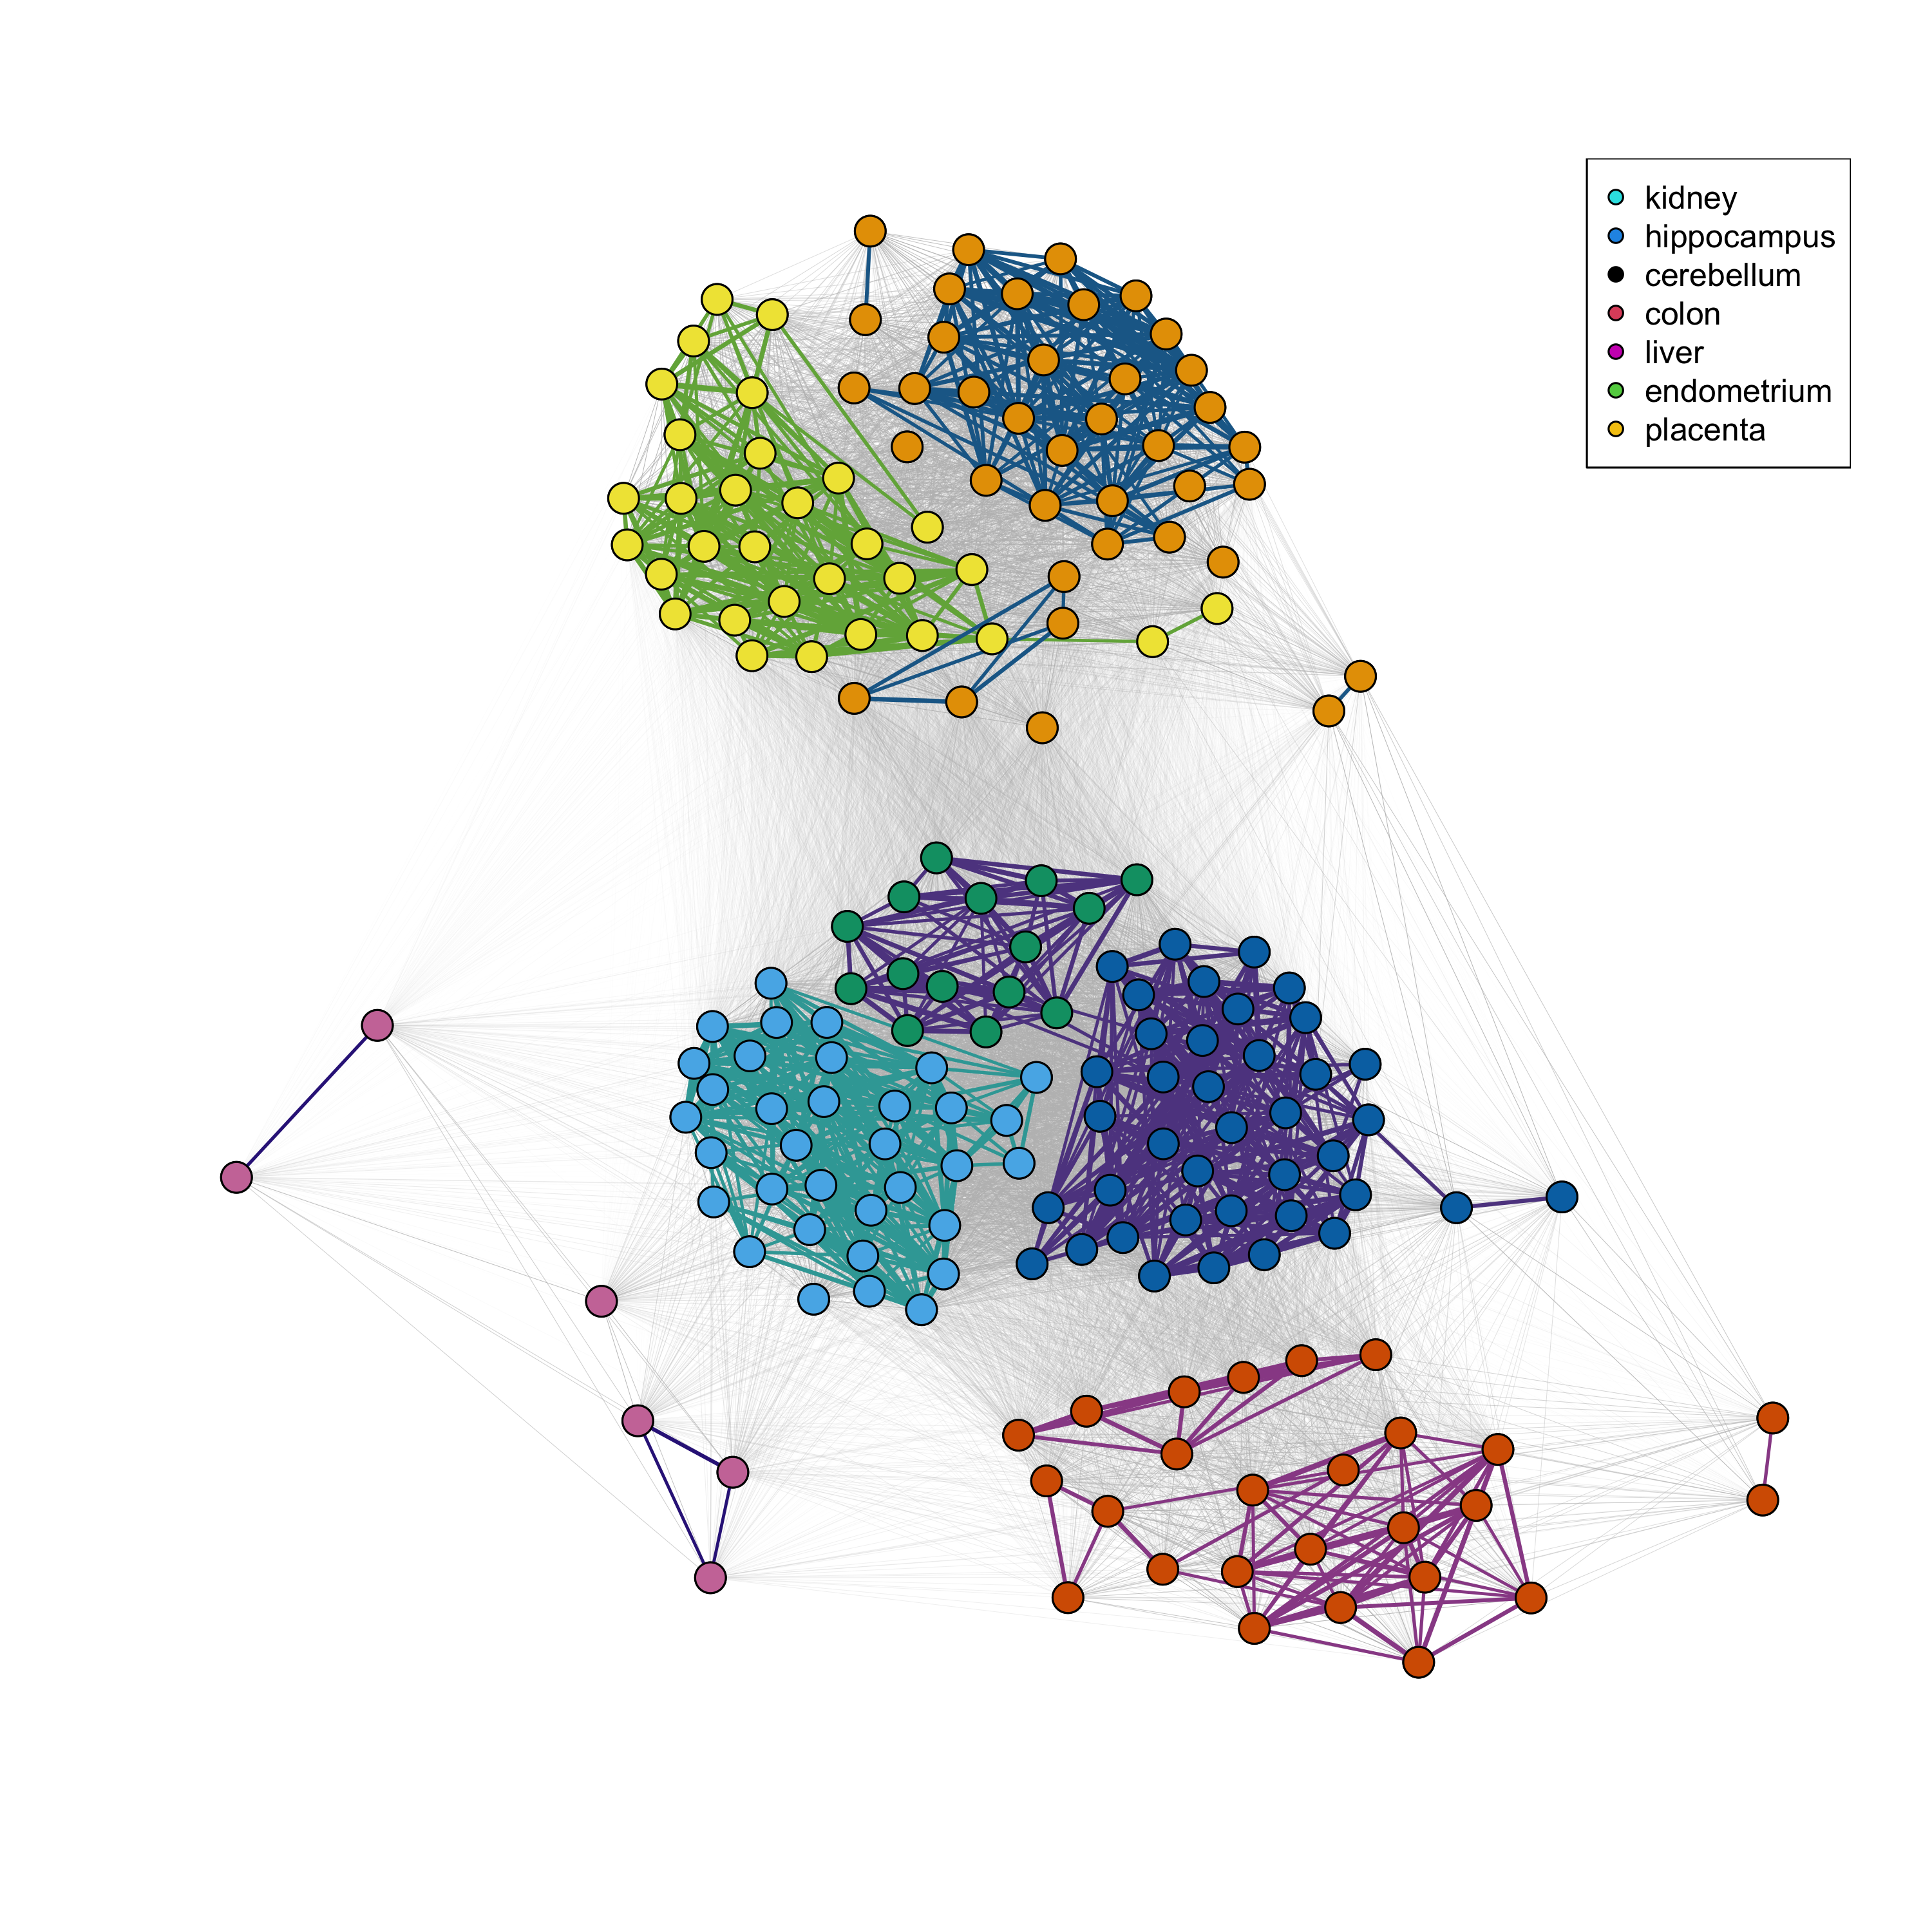
\includegraphics[width=5.5in,trim=0in 5in 0in 3in,clip]{fig5} \caption[Community cluster network for the tissue data]{Community cluster network for the tissue data. The line colors indicate the PaLD communities; the point colors indicate the tissue classification.}\label{fig:fig4}
\end{figure}
\end{Schunk}

A summary of community strong ties can be produced via the following
code. Note that \texttt{tissue\_graph\_strong} is an \CRANpkg{igraph}
object corresponding to the graph displayed in Figure \ref{fig:fig4},
restricted only to strong ties.

\begin{Schunk}
\begin{Sinput}
tissue_graphs <- community_graphs(tissue_cohesion)
tissue_graph_strong <- tissue_graphs[["G_strong"]]
E <- igraph::get.edgelist(tissue_graph_strong)
tissue_strong_ties <- data.frame(
  strong_ties = apply(E, 1, paste, collapse = ",")
)
tissue_strong_ties |>
  dplyr::count(strong_ties) |>
  dplyr::arrange(-n)
\end{Sinput}
\begin{Soutput}
#>               strong_ties   n
#> 1           kidney,kidney 273
#> 2             colon,colon 241
#> 3 hippocampus,hippocampus 191
#> 4   cerebellum,cerebellum 186
#> 5             liver,liver  85
#> 6 endometrium,endometrium  81
#> 7       placenta,placenta   4
#> 8      kidney,endometrium   3
\end{Soutput}
\end{Schunk}

Note that there are only three strong ties between different tissue
types (kidney and endometrium) in the community cluster network of 1,064
strong ties total.

\hypertarget{cognate-based-language-families}{%
\subsection{Cognate-based Language
Families}\label{cognate-based-language-families}}

This example explores a data set from \citet{dyen92} that summarizes
relationships between 87 Indo-European languages from the perspective of
cognates, coded using 2,655-dimensional binary vectors. A \texttt{dist}
object was created from this data set and is included in the
\CRANpkg{pald} package in an object called \texttt{cognate\_dist}.

Here we will demonstrate how one can further apply functions in the
\CRANpkg{igraph} package to objects output from the \CRANpkg{pald}
package. We can first use the \texttt{cohesion\_matrix} function to
calculate the cohesion matrix and the \texttt{community\_graphs}
function to create a list with the weighted community graph, the
weighted community graph with only strong ties included, and the layout.
From this, we can extract the graph with only the strong ties, here
called \texttt{cognate\_graph\_strong}.

\begin{Schunk}
\begin{Sinput}
cognate_cohesion <- cohesion_matrix(cognate_dist)
cognate_graphs <- community_graphs(cognate_cohesion)

cognate_graph_strong <- cognate_graphs[["G_strong"]]
\end{Sinput}
\end{Schunk}

We can then use the \texttt{neighbors} function from the
\CRANpkg{igraph} package to extract the strong neighbors in this graph.
For example, we can extract all neighbors for the language ``French'',
via the following code.

\begin{Schunk}
\begin{Sinput}
french_neighbors <- igraph::neighbors(cognate_graph_strong, "French")
french_neighbors
\end{Sinput}
\begin{Soutput}
#> + 8/87 vertices, named, from b09505b:
#> [1] Italian         Ladin           Provencal       Walloon
#> [5] French_Creole_C French_Creole_D Spanish         Catalan
\end{Soutput}
\end{Schunk}

Similarly, we can sort and print the associated neighborhood weights by
subsetting the cohesion matrix.

\begin{Schunk}
\begin{Sinput}
cognate_cohesion["French", french_neighbors] |>
  sort(decreasing = TRUE)
\end{Sinput}
\begin{Soutput}
#>         Walloon       Provencal French_Creole_C French_Creole_D           Ladin
#>      0.03258771      0.02871174      0.02406057      0.02406057      0.02094596
#>         Italian         Catalan         Spanish
#>      0.01997696      0.01859688      0.01679733
\end{Soutput}
\end{Schunk}

We can again use the \texttt{plot\_community\_graphs} function to
visualize the community clusters (Figure \ref{fig:figlang}). One may
note the commonly identifiable language clusters and that, under a
slight rotation, some of the underlying geography is mirrored in the
plot.

\begin{Schunk}
\begin{Sinput}
plot_community_graphs(
  cognate_cohesion,
  edge_width_factor = 30,
  emph_strong = 3,
  vertex.size = 3,
  vertex.label.cex = 0.7,
  vertex.label.dist = 1
)
\end{Sinput}
\end{Schunk}

\begin{Schunk}
\begin{figure}[H]
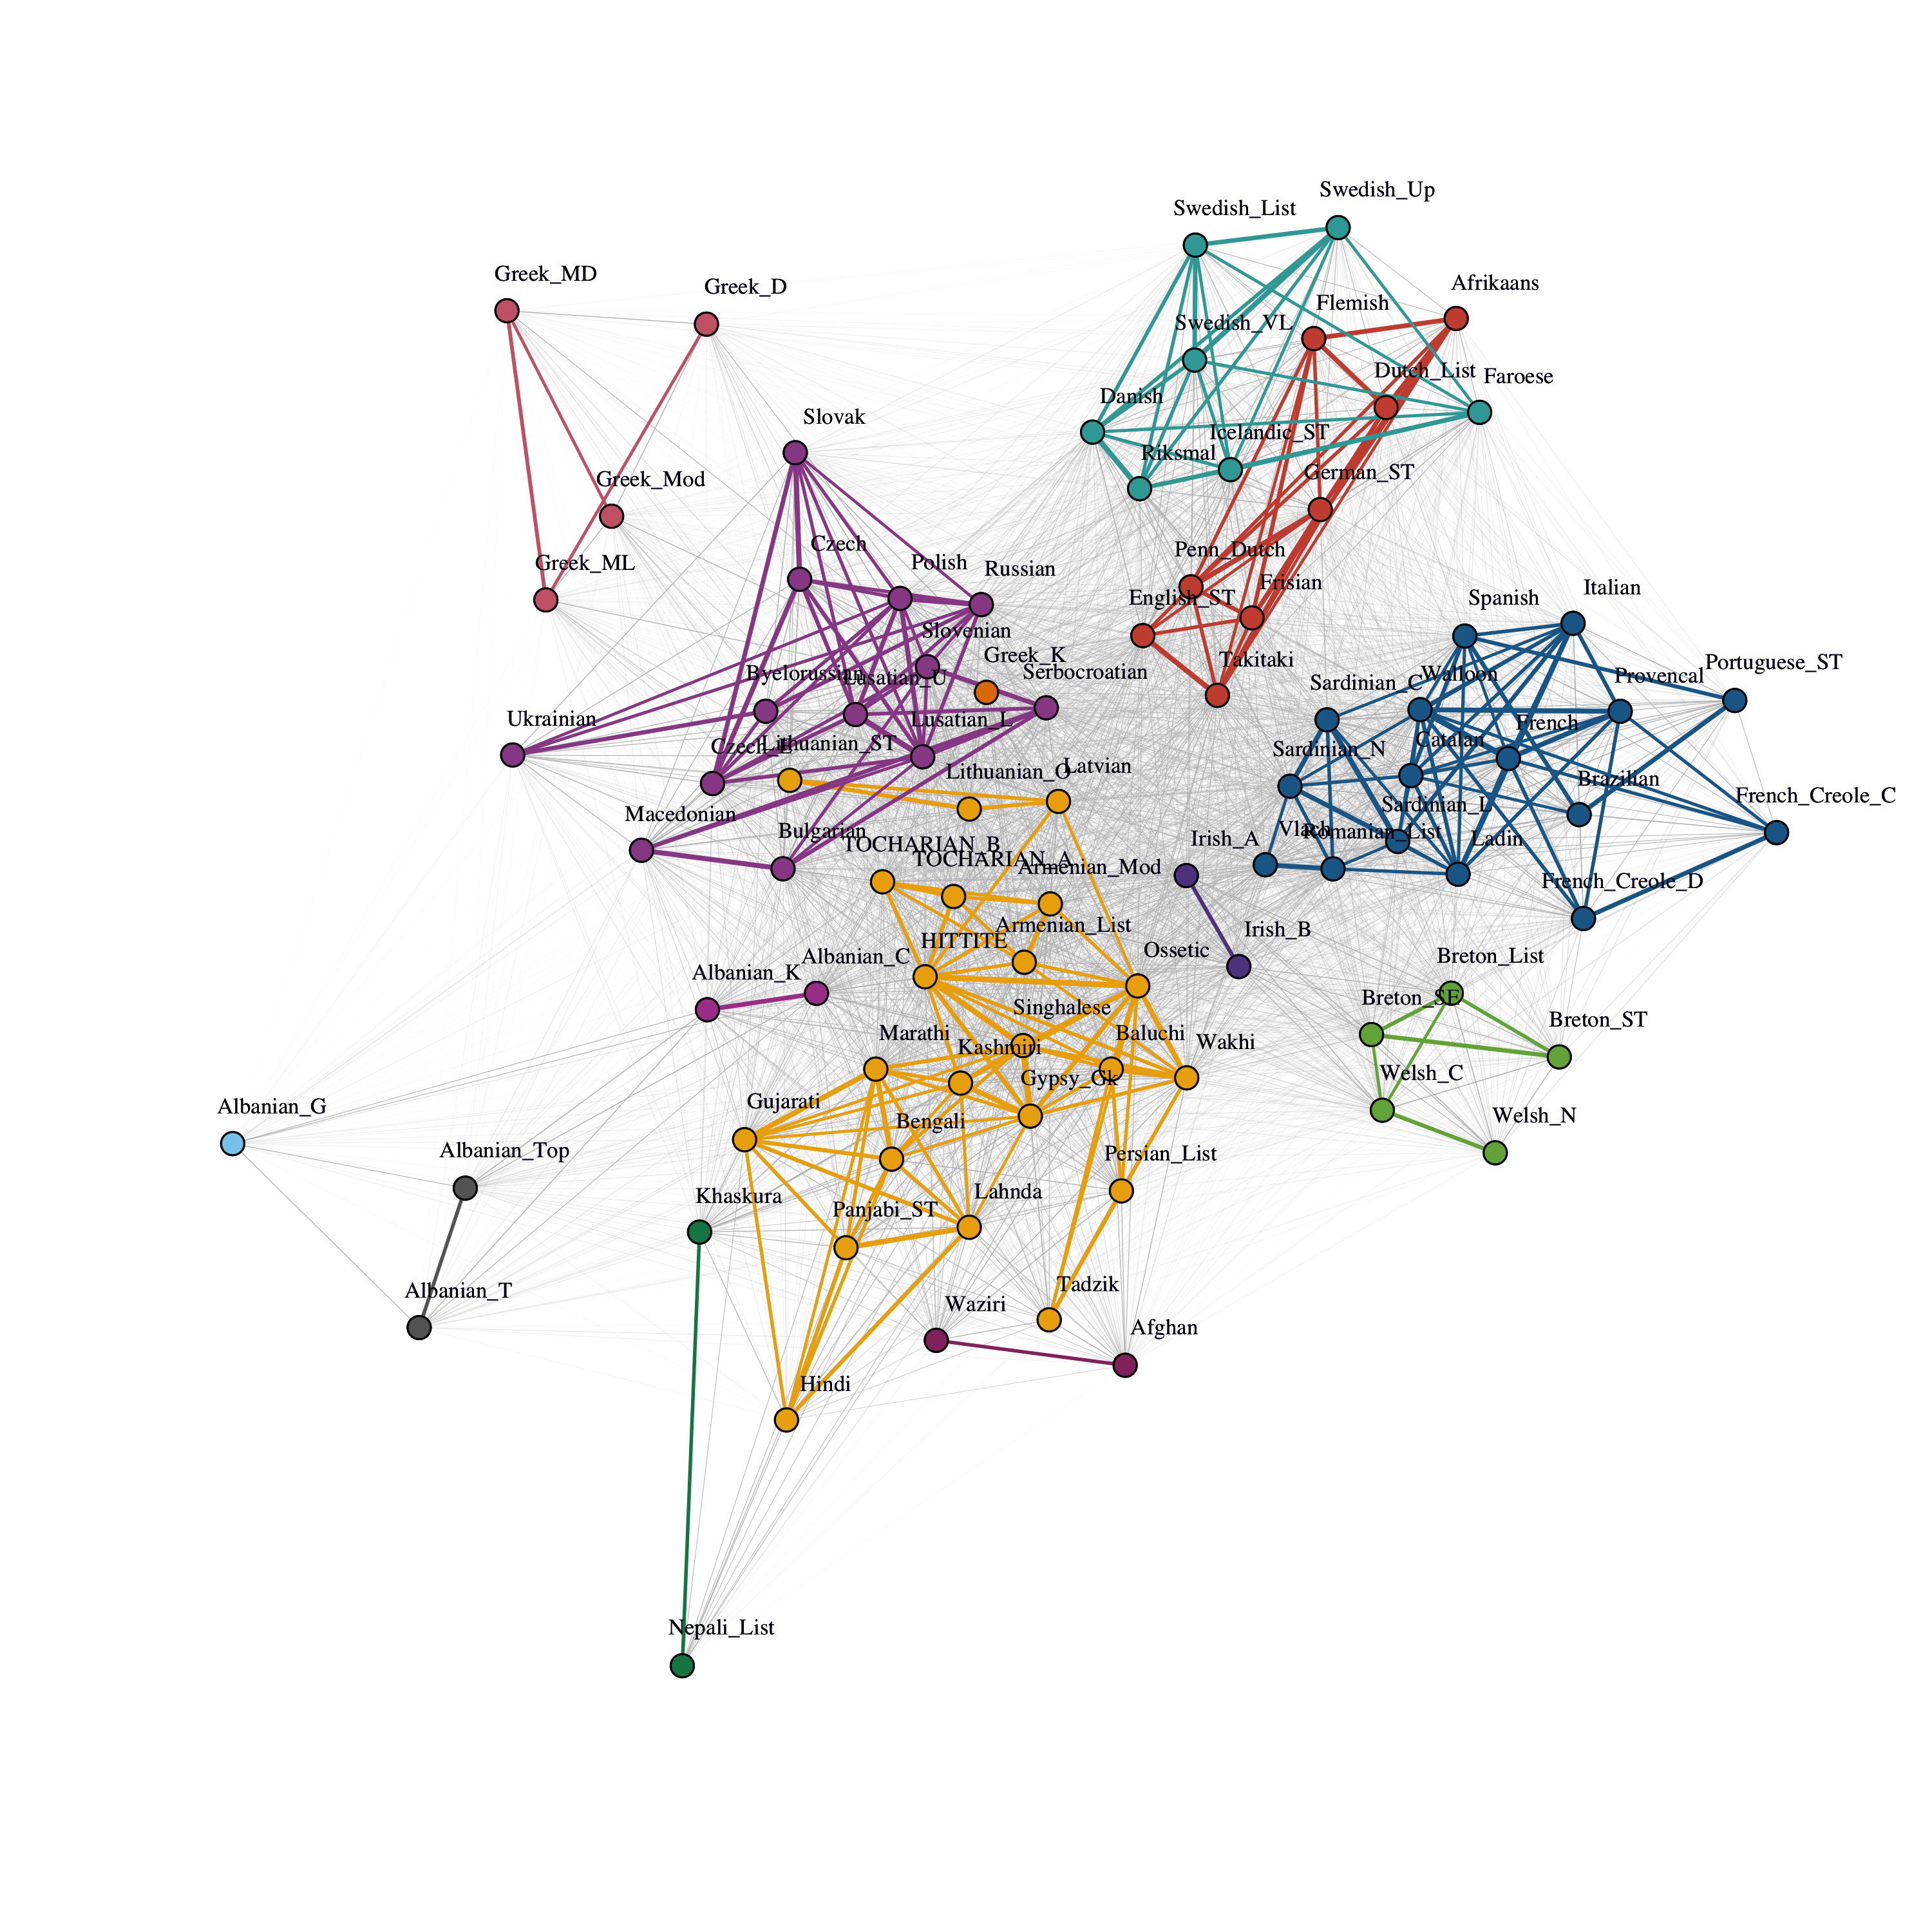
\includegraphics[width=5.5in,trim=0in 5in 0in 1in,clip]{fig6} \caption[Community structure for 87 Indo-European languages, which employs cognate information that was coded via 2,665-dimensional binary vectors]{Community structure for 87 Indo-European languages, which employs cognate information that was coded via 2,665-dimensional binary vectors. Commonly identifiable language clusters arise along with informative inter- and intra-cluster structure. Several ancient languages are centrally located.}\label{fig:figlang}
\end{figure}
\end{Schunk}

\hypertarget{community-analysis-for-generated-data}{%
\subsubsection{Community analysis for generated
data}\label{community-analysis-for-generated-data}}

The \CRANpkg{pald} package includes three randomly generated data frames
corresponding to plots from \citet{berenhaut2022social}:

\begin{itemize}
\tightlist
\item
  \texttt{exdata1} is a data set consisting of 8 points used to create
  Figure 1 in \citet{berenhaut2022social}
\item
  \texttt{exdata2} is a data set consisting of 16 points used to create
  Figure 2 in \citet{berenhaut2022social}
\item
  \texttt{exdata3} is a data set consisting of 240 points used to create
  Figure 4D in \citet{berenhaut2022social}
\end{itemize}

Here, we will demonstrate how to use \texttt{exdata3}. These points were
generated from bivariate normal distributions with varying means and
variances. There are eight ``true'' communities.

We will contrast community analysis via PaLD to standard cluster
analysis by considering two common clustering methods. The code below
calculates the cohesion matrix (\texttt{exdata\_cohesion}) as well as
the community clusters obtained via PaLD (\texttt{exdata\_pald}), along
with \(k=8\) clusters obtained via \emph{k}-means
(\texttt{exdata\_kmeans}) and hierarchical clustering using complete
linkage (\texttt{exdata\_hclust}). Recall that there is no need to
determine values for extraneous inputs in the case of PaLD (e.g.~the
number of clusters, as is necessary to specify for \emph{k}-means and
hierarchical clustering).

\begin{Schunk}
\begin{Sinput}
exdata_cohesion <- exdata3 |>
  dist() |>
  cohesion_matrix()

exdata_pald <- community_clusters(exdata_cohesion)$community

exdata_kmeans <- kmeans(exdata3, 8)$cluster

exdata_hclust <- exdata3 |>
  dist() |>
  hclust() |>
  cutree(k = 8)
\end{Sinput}
\end{Schunk}

The information is displayed in Figure \ref{fig:fig5}.

\begin{Schunk}
\begin{Sinput}
par(mfrow = c(1, 3), pty = "s")
plot(
  exdata3,
  pch = 16,
  col = pald_colors[exdata_pald],
  xlab = "",
  ylab = "",
  main = "PaLD Communities",
  asp = 1
)
plot(
  exdata3,
  pch = 16,
  col = pald_colors[exdata_kmeans],
  xlab = "",
  ylab = "",
  main = "K-Means Clusters (k = 8)",
  asp = 1
)
plot(
  exdata3,
  pch = 16,
  col = pald_colors[exdata_hclust],
  xlab = "",
  ylab = "",
  main = "Hiearchical Clusters (k = 8)",
  asp = 1
)
\end{Sinput}
\begin{figure}[H]
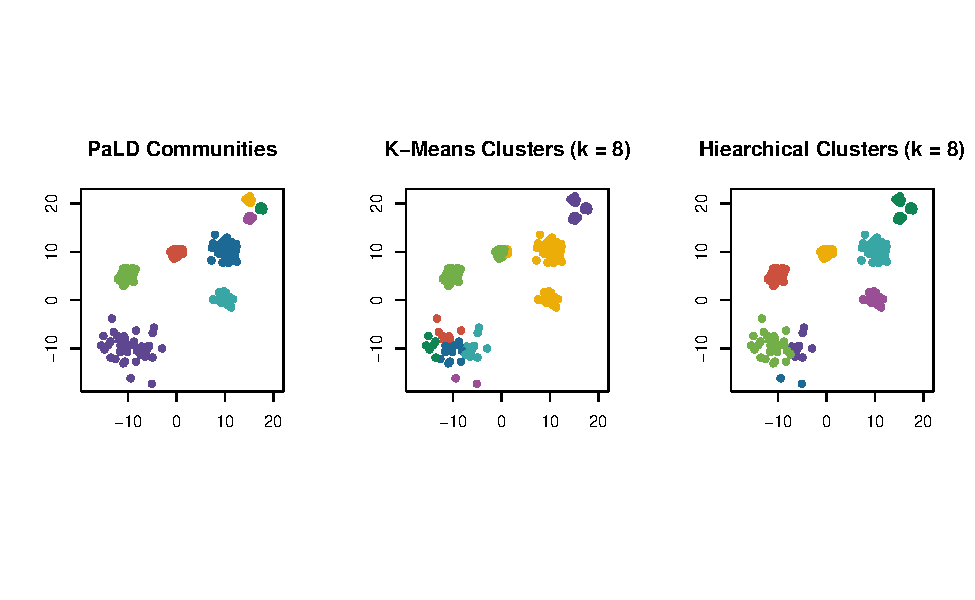
\includegraphics[width=5.5in,trim=0in 1in 0in 0.8in,clip]{dagostino-mcgowan_files/figure-latex/fig5-1} \caption[PaLD, k-means, and hierarchical 8-clustering of randomly generated example data (from \citet{berenhaut2022social}]{PaLD, k-means, and hierarchical 8-clustering of randomly generated example data (from \citet{berenhaut2022social}; Figure 4D).}\label{fig:fig5}
\end{figure}
\end{Schunk}

Cohesion is particularly useful when considering data with varying local
density; see \citet{berenhaut2022social} for further examples,
discussion, and theoretical results. Note that the PaLD algorithm is
able to detect the eight natural groups within the data (along with
inter- and intra-community structure not displayed here) without the use
of any additional inputs (e.g., number of clusters) nor optimization
criteria. Despite the user input of the ``correct'' number of clusters
(i.e., \(k = 8\)) both \emph{k}-means and hierarchical clustering do not
provide the desired result.

\hypertarget{cultural-and-pyschological-distance-analysis}{%
\subsubsection{Cultural and Pyschological distance
analysis}\label{cultural-and-pyschological-distance-analysis}}

In this example we perform a PaLD analysis for cultural distances
obtained in \citet{muthukrishna2020beyond} from two recent waves of the
World Values Survey (2005 to 2009 and 2010 to 2014; see
\citet{inglehart2014world}). Distances are computed using the cultural
fixation index (CFST), which is a measure built on the framework of
fixation indices from population biology
(\citet{bell2009culture,cavalli1994history}). Recall that the foundation
of PaLD in within-triplet comparisons allows for the employment of
application-dependent and non-Euclidean measures of dissimilarity. The
\texttt{dist} object is included in the \CRANpkg{pald} package
(\texttt{cultures}). We will first create the cohesion matrix using the
\texttt{dist} object \texttt{cultures}, and proceed to plot the
community graph.

\begin{Schunk}
\begin{Sinput}
cultures_cohesion <- cohesion_matrix(cultures)
\end{Sinput}
\end{Schunk}

\begin{Schunk}
\begin{Sinput}
plot_community_graphs(
  cultures_cohesion,
  edge_width_factor = 30,
  emph_strong = 3,
  vertex.label.cex = 0.7,
  vertex.size = 3,
  vertex.label.dist = 1
)
\end{Sinput}
\end{Schunk}

\begin{Schunk}
\begin{figure}[H]
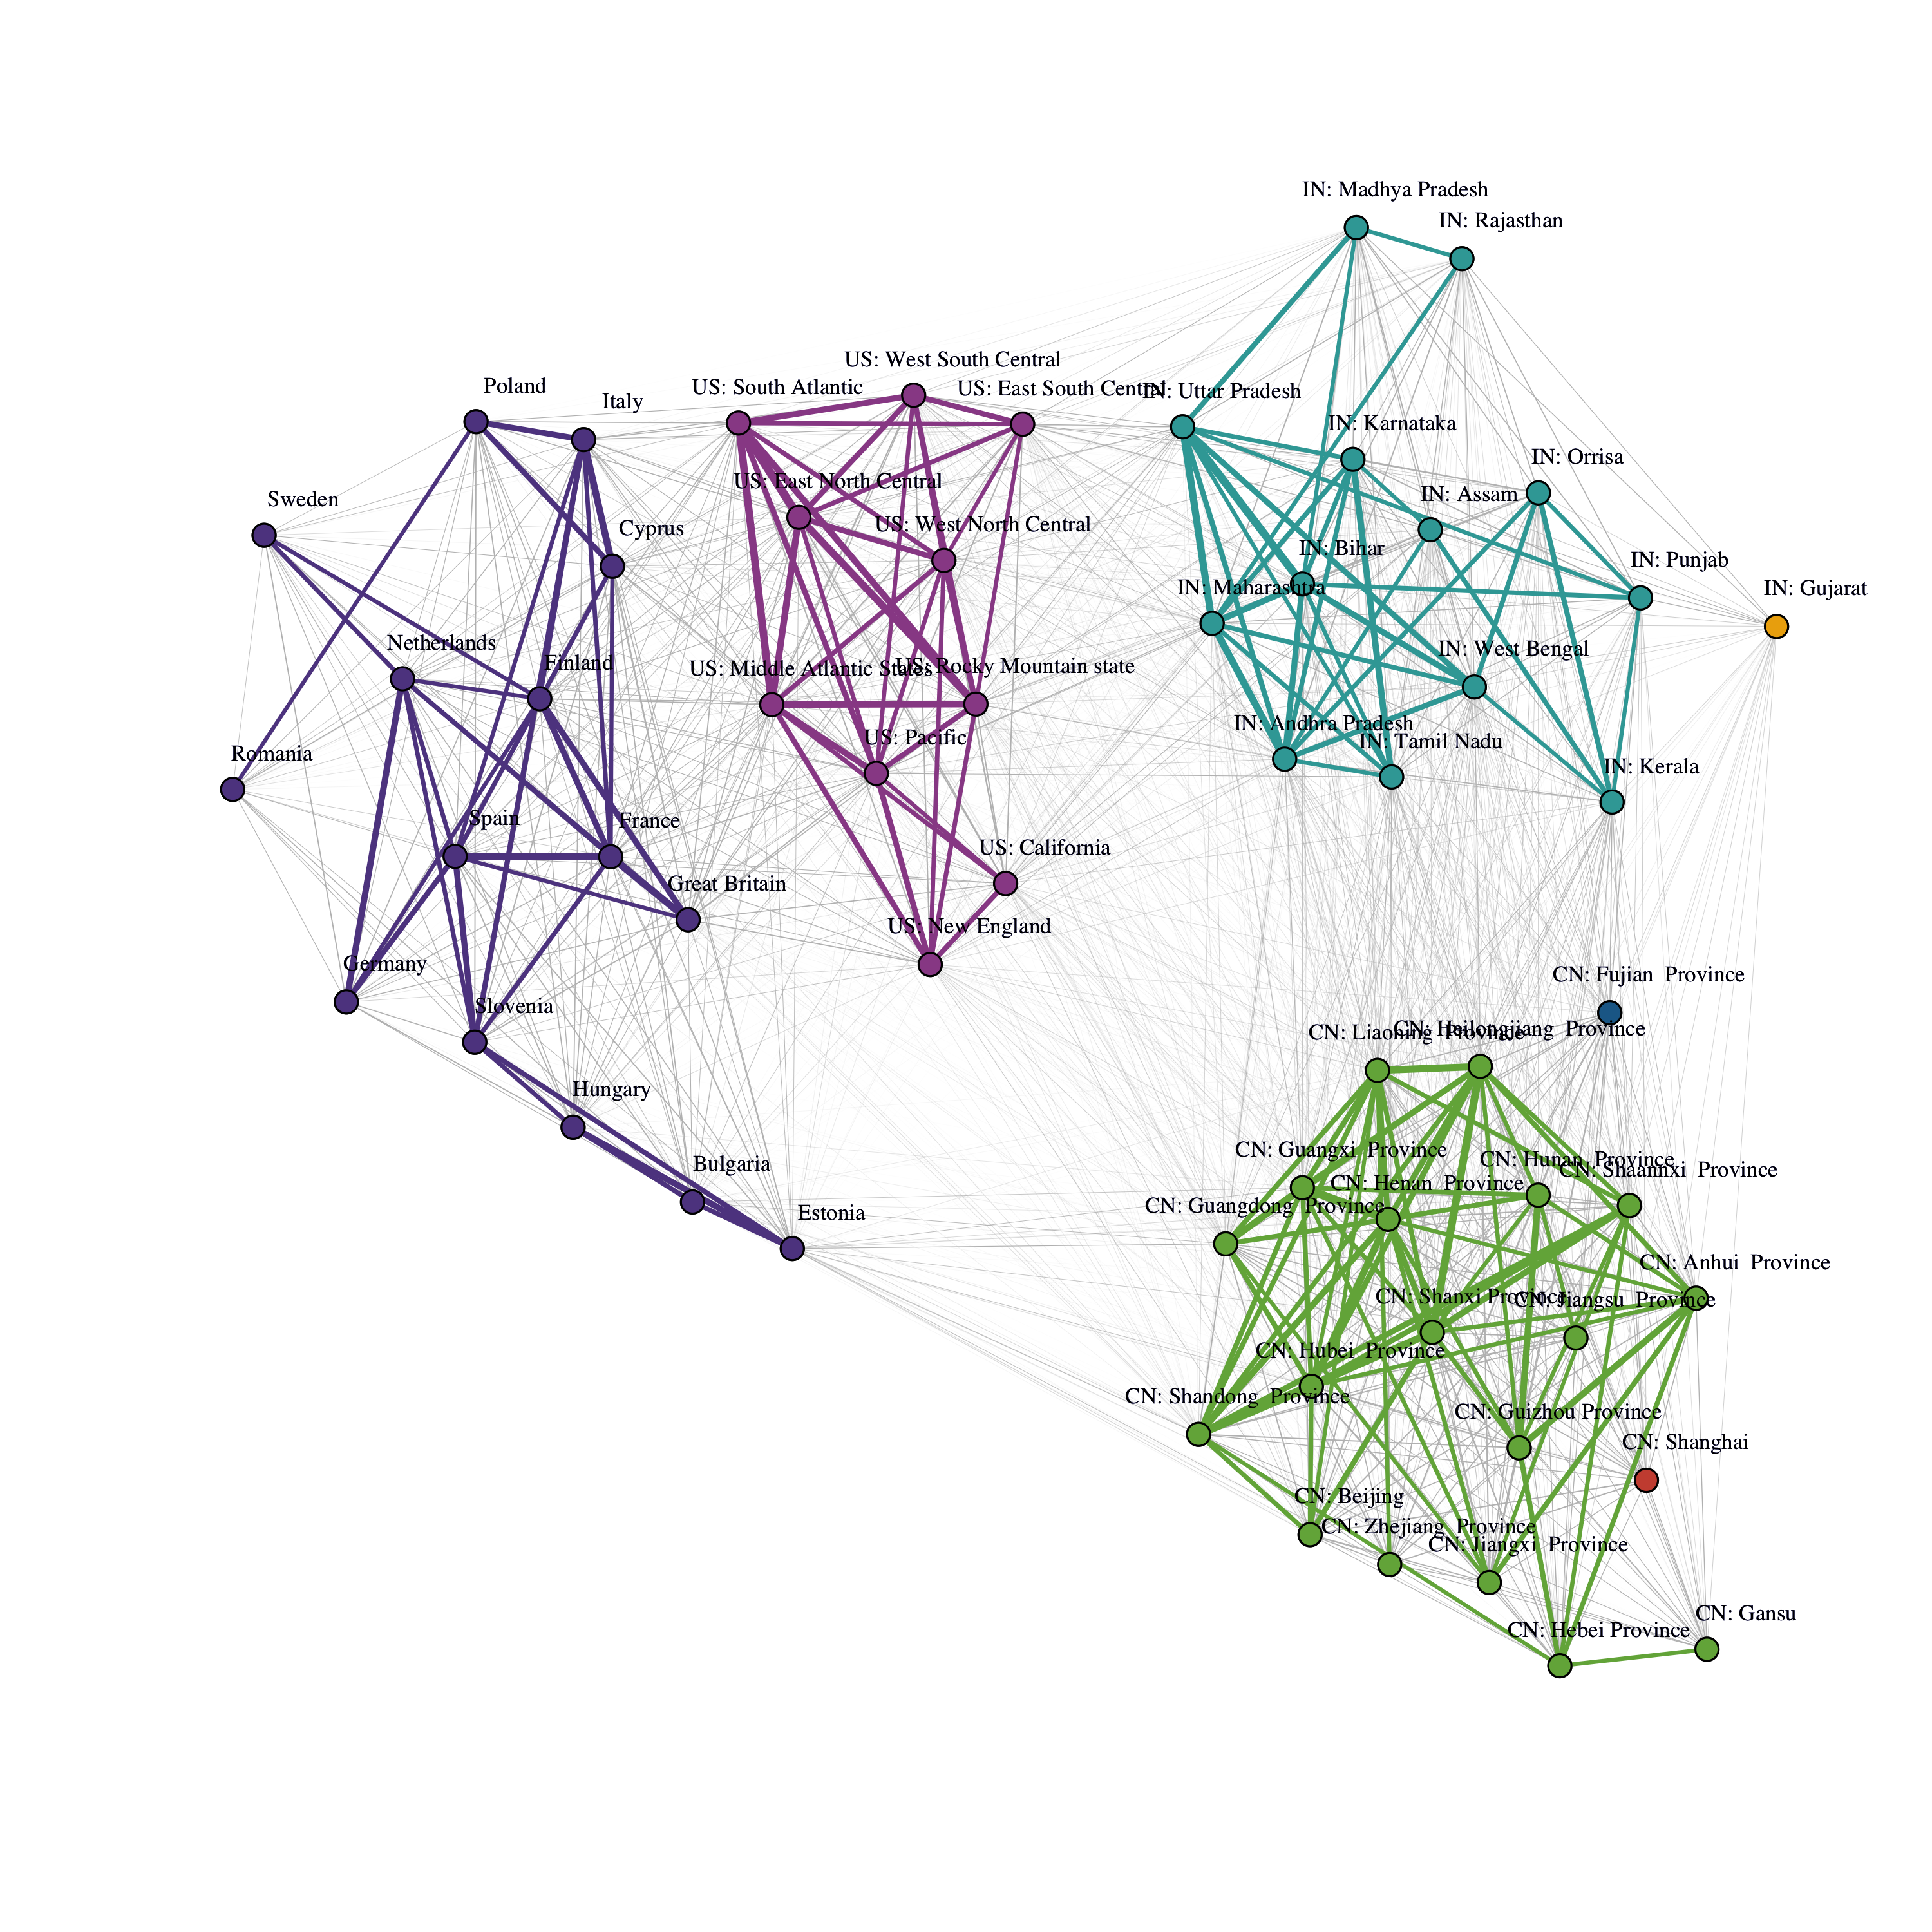
\includegraphics[width=5.5in,trim=0in 5in 0in 3in,clip]{fig7} \caption[Community structure for cultural distance data]{Community structure for cultural distance data.}\label{fig:figculture}
\end{figure}
\end{Schunk}

In addition to viewing the local and global community structure as seen
in Figure \ref{fig:figculture}, the \CRANpkg{pald} package allows for a
two-dimensional display of cohesion against distance for the data, via
the \texttt{dist\_cohesion\_plot} function, as seen below (Figure
\ref{fig:figco}).

\begin{Schunk}
\begin{Sinput}
dist_cohesion_plot(cultures, mutual = TRUE)
\end{Sinput}
\begin{figure}[H]
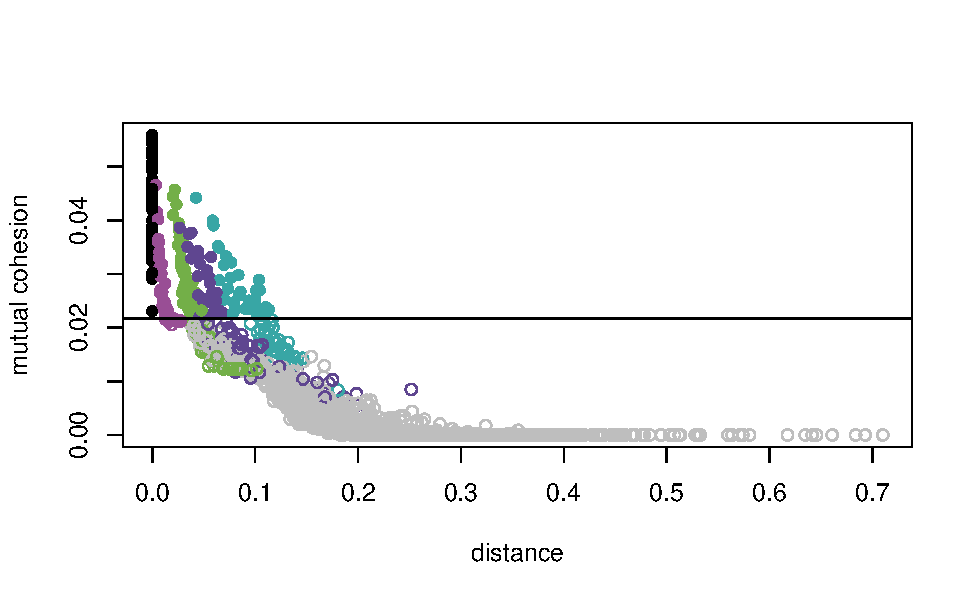
\includegraphics[width=5.5in,trim=0in 0.5in 0in 0.5in,clip]{dagostino-mcgowan_files/figure-latex/figco-1} \caption{A plot of cohesion versus distance for the data. The identified communities are colored as in Figure \ref{fig:figculture}.}\label{fig:figco}
\end{figure}
\end{Schunk}

Notice here that the magnitude of the distances within each of the
identified communities varies substantially between regions; in fact,
the most disparate two regions in the United States (at distance
\(\approx\) 0.027) are far closer than the two most similar in India (at
distance \(\approx\) 0.043). Despite this, India remains a cohesive
whole, and locally disparate regions in the United States such as East
South Central and California are not strongly cohesive. For discussion
of subtleties in local density (see \citet{berenhaut2022social}.
Additionally, currently available techniques require specification of
parameters, as seen in the previous section. For further discussion of
the cultural distance data in relation to community analysis see
\citet{berenhaut2022social}.

\hypertarget{summary}{%
\subsection{Summary}\label{summary}}

This paper introduces the \CRANpkg{pald} package, demonstrating its
utility for providing novel parameter-free community analysis which can
easily be implemented for a variety of data sets, supplementing results
from other methods for clustering, embedding, nearest neighbors, etc.
Example code is provided along with discussion in the context of other
commonly used R-based approaches.

\bibliography{RJreferences}


\address{%
Lucy D'Agostino McGowan\\
Wake Forest University\\%
Winston-Salem, NC\\ 27106\\
%
%
%
\href{mailto:mcgowald@wfu.edu}{\nolinkurl{mcgowald@wfu.edu}}%
}

\address{%
Katherine Moore\\
Amherst College\\%
Amherst, MA\\ 1002\\
%
%
%
\href{mailto:kmoore@amherst.edu}{\nolinkurl{kmoore@amherst.edu}}%
}

\address{%
Kenneth Berenhaut\\
Wake Forest University\\%
Winston-Salem, NC\\ 27106\\
%
%
%
\href{mailto:berenhks@wfu.edu}{\nolinkurl{berenhks@wfu.edu}}%
}
